\begin{figure}[!htbp]
\centering
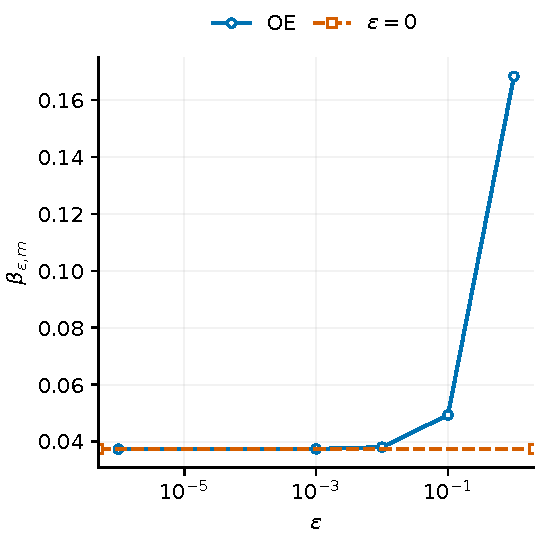
\includegraphics[width=0.75\linewidth]{figures/fig01.pdf}
\caption{Fixed-space minimum gain $\beta_{\varepsilon,m}^{(q)}$ on the 32-dimensional parity-conforming space with seed 11 and no singular-value truncation. The horizontal line marks the value evaluated at $\varepsilon=0$; positive $\varepsilon$ values are shown on the logarithmic axis. This diagnostic uses its own $H^1\times H^1$ and unweighted inflow norms and refined quadrature; it does not verify Assumption~1 for the main experiment configurations.}
\label{fig:minimum-gain}
\end{figure}

\begin{figure}[!htbp]
\centering
\begin{minipage}{.45\linewidth}\centering
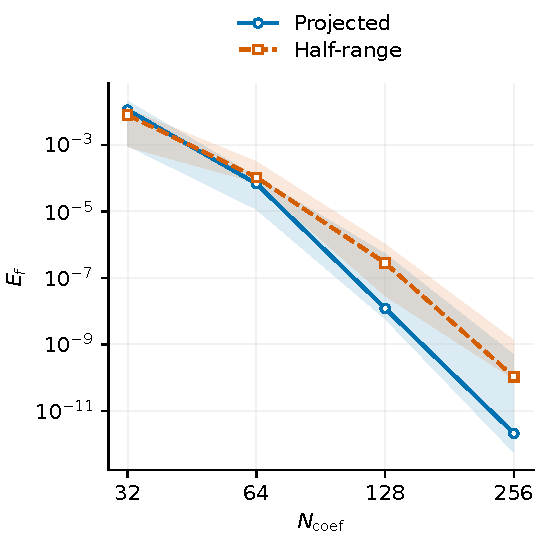
\includegraphics[width=0.90\linewidth]{figures/fig02a.pdf}
\end{minipage}\hfill
\begin{minipage}{.45\linewidth}\centering
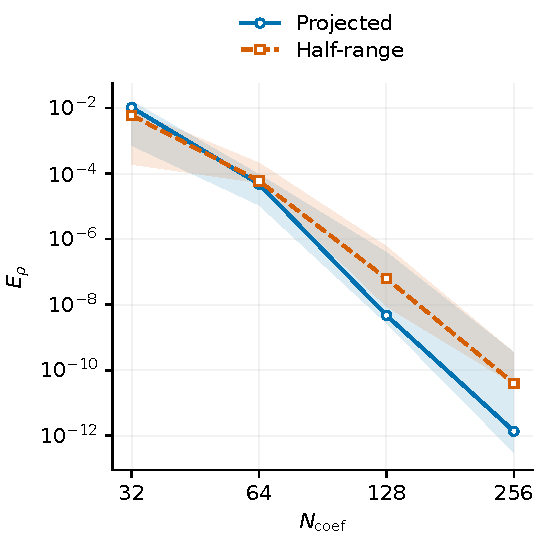
\includegraphics[width=0.90\linewidth]{figures/fig02b.pdf}
\end{minipage}
\caption{Projected-basis versus unprojected positive-half-range approximation at $\varepsilon=10^{-3}$: relative kinetic error (left) and relative density error (right).
Curves show medians over three random seeds, with shaded bands indicating the minimum and maximum.
Both reconstructions have even $r_h$ and odd $j_h$; the unprojected control uses $f_h(x,v)=\widetilde r_h(x,|v|)+\varepsilon\operatorname{sgn}(v)\widetilde j_h(x,|v|)$, consistent with training. The legend labels these spaces as Projected and Half-range. Coefficient and residual counts are matched within each budget, not across budgets. This compares basis constructions, not the presence or absence of physical parity.}
\label{fig:parity-budget}
\end{figure}

\begin{figure}[!htbp]
\centering
\begin{minipage}{.45\linewidth}\centering
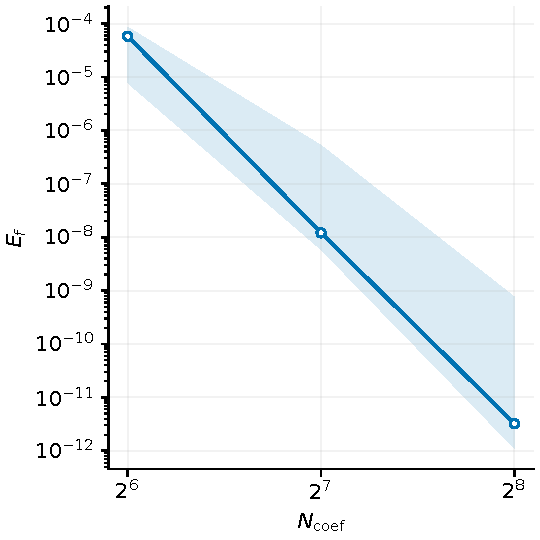
\includegraphics[width=0.90\linewidth]{figures/fig03a.pdf}
\end{minipage}\hfill
\begin{minipage}{.45\linewidth}\centering
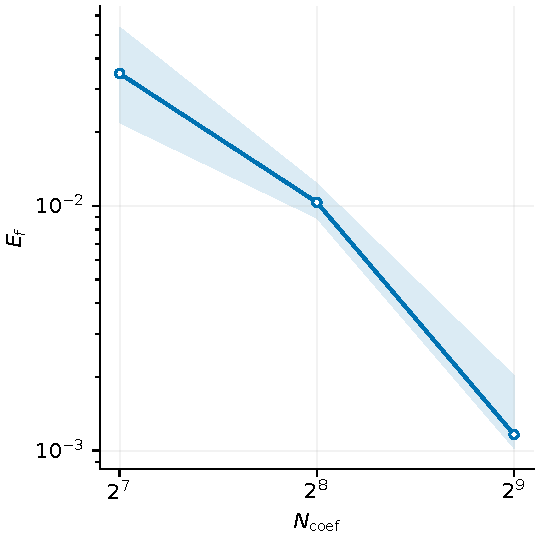
\includegraphics[width=0.90\linewidth]{figures/fig03b.pdf}
\end{minipage}
\caption{Feature refinement at fixed collocation and $\varepsilon=10^{-3}$: one-dimensional manufactured transport with 2944 rows (left) and the four-component two-dimensional problem with 13808 rows (right). Numerical values, density errors, and effective-rank fractions are reported in Table \ref{tab:feature-resolution}.}
\label{fig:feature-resolution}
\end{figure}

\begin{figure}[!htbp]
\centering
\begin{subfigure}[t]{0.32\linewidth}
\centering
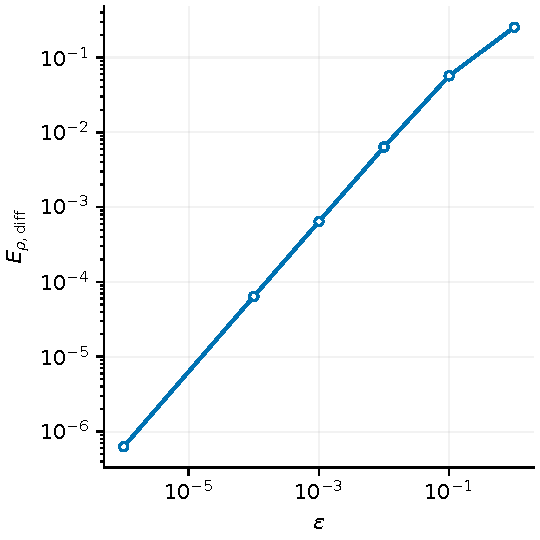
\includegraphics[width=\linewidth]{figures/fig04a.pdf}
\caption{Density error.}
\end{subfigure}
\hfill
\begin{subfigure}[t]{0.32\linewidth}
\centering
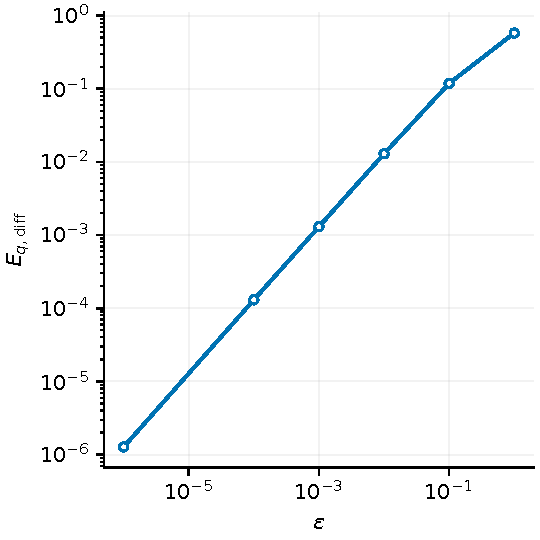
\includegraphics[width=\linewidth]{figures/fig04b.pdf}
\caption{Scaled-flux error.}
\end{subfigure}
\hfill
\begin{subfigure}[t]{0.32\linewidth}
\centering
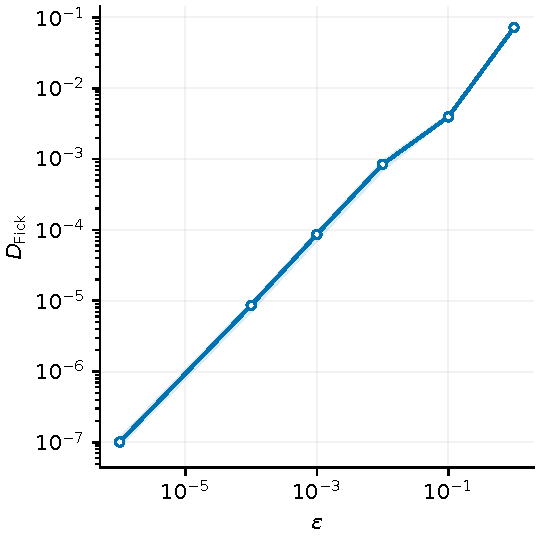
\includegraphics[width=\linewidth]{figures/fig04c.pdf}
\caption{Fick defect.}
\end{subfigure}
\caption{The diffusion-limit behavior for steady slab transport. The left and center panels show the relative differences of the numerical density and scaled flux from their diffusion-limit counterparts, while the right panel shows the interior Fick defect. The data and numerical discretization are held fixed throughout the $\varepsilon$ sweep. The evidence applies to this slab configuration.}
\label{fig:steady-diffusion}
\end{figure}

\begin{figure}[!htbp]
\centering
\begin{minipage}{.45\linewidth}\centering
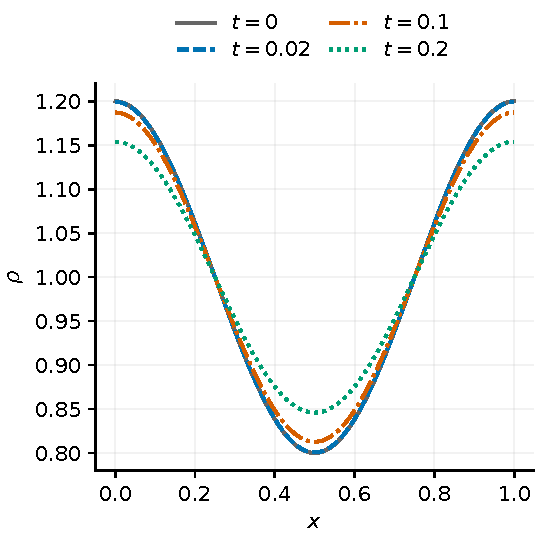
\includegraphics[width=0.90\linewidth]{figures/fig05a.pdf}
\end{minipage}\hfill
\begin{minipage}{.45\linewidth}\centering
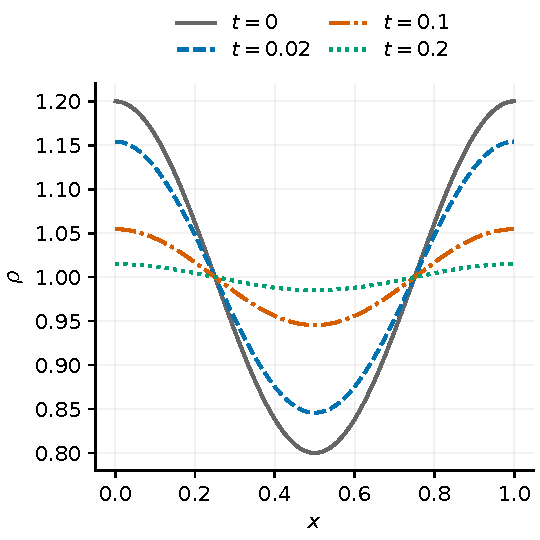
\includegraphics[width=0.90\linewidth]{figures/fig05b.pdf}
\end{minipage}
\par\smallskip
\begin{minipage}{.45\linewidth}\centering
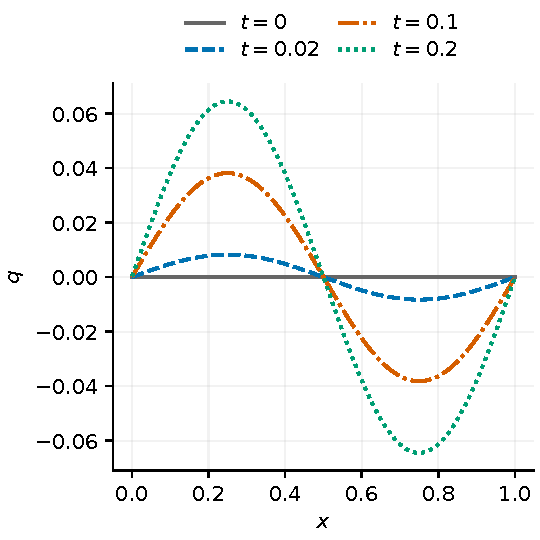
\includegraphics[width=0.90\linewidth]{figures/fig05c.pdf}
\end{minipage}\hfill
\begin{minipage}{.45\linewidth}\centering
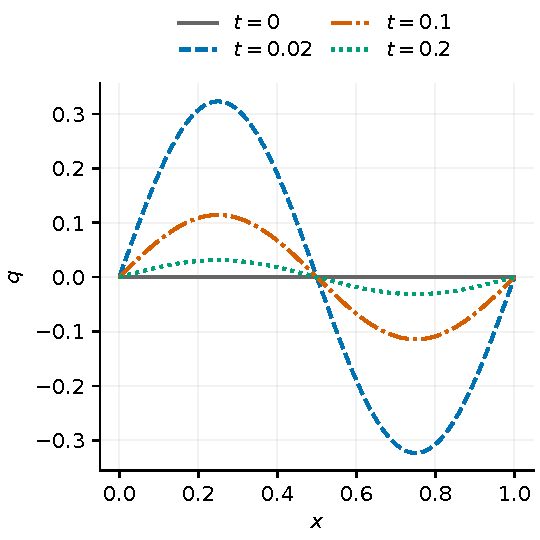
\includegraphics[width=0.90\linewidth]{figures/fig05d.pdf}
\end{minipage}
\caption{Density and scaled-flux evolution for periodic
transport with seed 11 and $\Delta t=0.002$.
Columns correspond to $\varepsilon=1$ (left)
and $10^{-3}$ (right); rows show density (top)
and scaled flux (bottom) at
$t=0,0.02,0.10,0.20$. The $t=0$ fields are the analytic initial data, not a random-feature fit; the first step uses these analytic data directly.}
\label{fig:transient-evolution}
\end{figure}

\begin{figure}[!htbp]
\centering
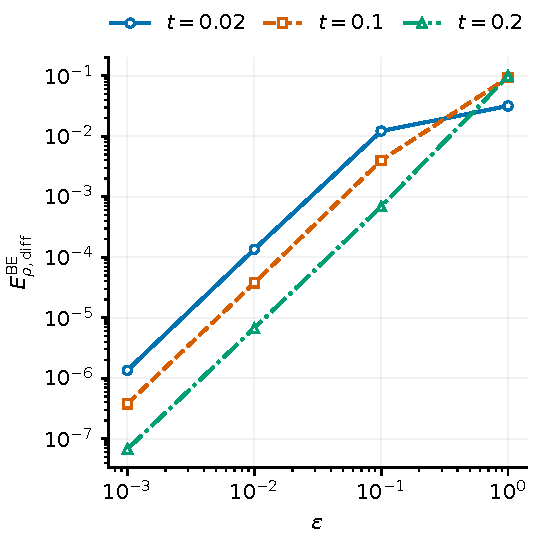
\includegraphics[width=0.75\linewidth]{figures/fig06.pdf}
\caption{Time-discrete diffusion limit for periodic transport at $\Delta t=0.002$.
The data, spatial discretization and time step are fixed throughout this sweep. The ordinate is the relative density difference from the backward-Euler diffusion solution in Equation \eqref{eq:transient-diffusion-reference}.}
\label{fig:transient-diffusion}
\end{figure}

\begin{figure}[!htbp]
\centering
\begin{subfigure}[t]{0.32\linewidth}
\centering
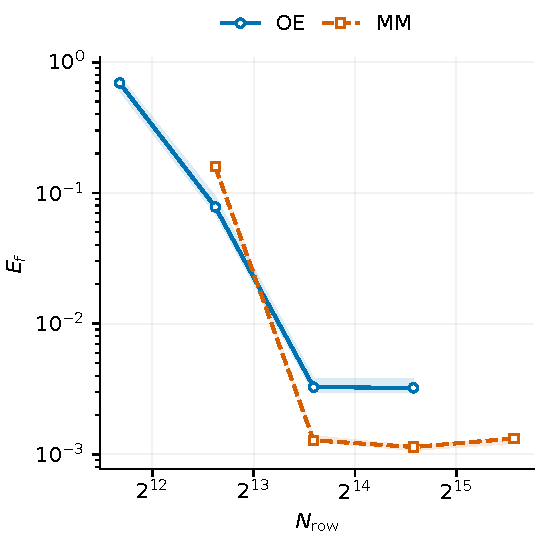
\includegraphics[width=\linewidth]{figures/fig07a.pdf}
\caption{Kinetic error.}
\end{subfigure}
\hfill
\begin{subfigure}[t]{0.32\linewidth}
\centering
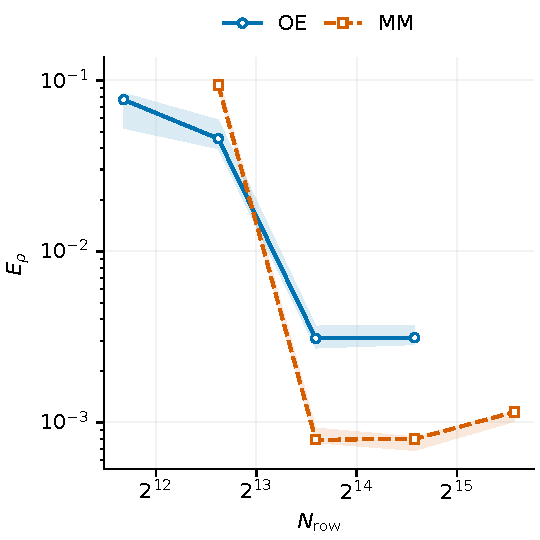
\includegraphics[width=\linewidth]{figures/fig07b.pdf}
\caption{Density error.}
\end{subfigure}
\hfill
\begin{subfigure}[t]{0.32\linewidth}
\centering
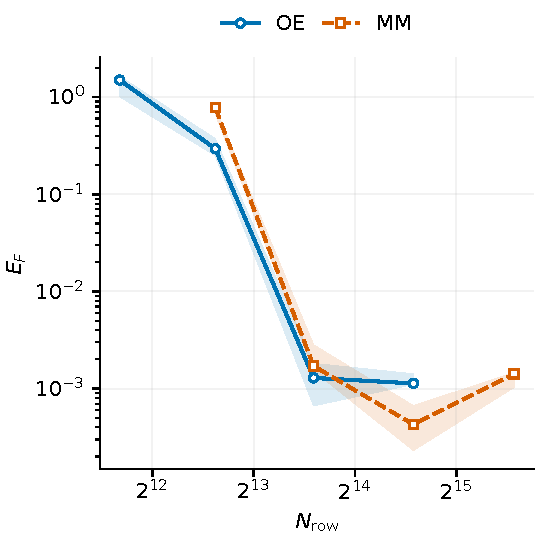
\includegraphics[width=\linewidth]{figures/fig07c.pdf}
\caption{Physical-flux error.}
\end{subfigure}
\caption{Differences from an archived transport reference for the one-dimensional mixed-scale problem, as functions of $N_{\rm row}$. Reference-accuracy diagnostics on the main evaluation grid did not meet the prescribed acceptance criterion for all configurations. These results examine budget dependence and are excluded from the main accuracy claims and fine method rankings.
Curves show three-seed medians, with bands spanning the minimum and maximum.}
\label{fig:mixed-budget}
\end{figure}

\begin{figure}[!htbp]
\centering
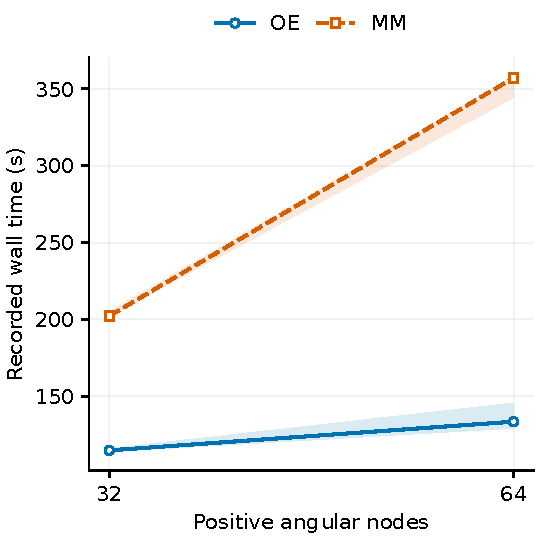
\includegraphics[width=0.75\linewidth]{figures/fig08.pdf}
\caption{Computation time versus positive-angle budget for the one-dimensional mixed-scale problem with seed 11.
Points show medians over three independent process runs, with bands spanning the minimum and maximum. They are not combined with the uncertified reference-relative differences to claim an equal-accuracy speedup.}
\label{fig:mixed-timing}
\end{figure}

\begin{figure}[!htbp]
\centering
\begin{subfigure}[t]{0.45\linewidth}
\centering
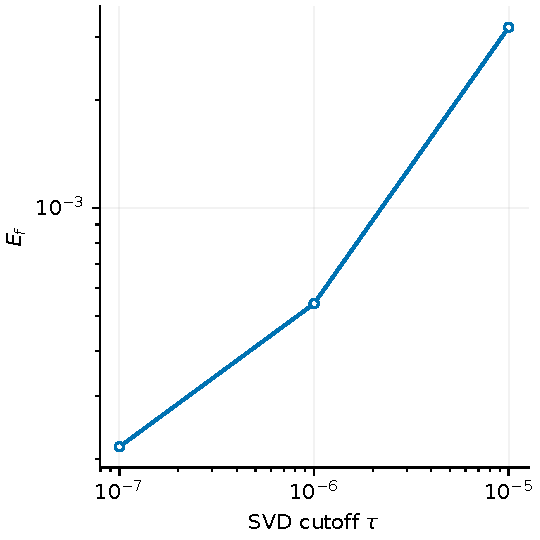
\includegraphics[width=0.90\linewidth]{figures/fig09a.pdf}
\caption{Kinetic error.}
\end{subfigure}
\hfill
\begin{subfigure}[t]{0.45\linewidth}
\centering
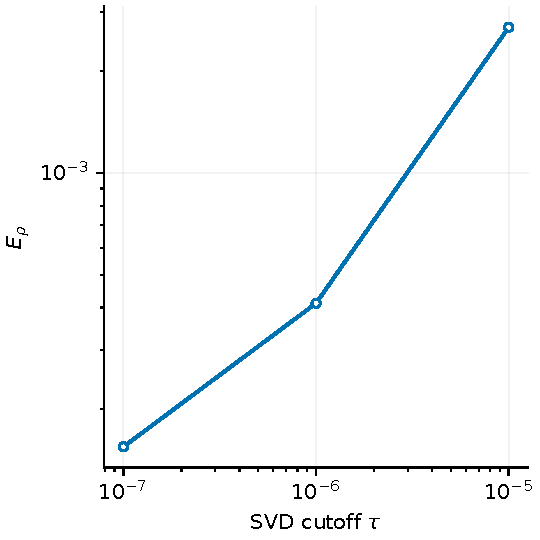
\includegraphics[width=0.90\linewidth]{figures/fig09b.pdf}
\caption{Density error.}
\end{subfigure}
\caption{Sensitivity to the relative SVD cutoff for the two-dimensional variable-scattering problem at $\varepsilon=10^{-3}$: kinetic error (left) and density error (right). All entries use seed 11, 1024 coefficients, 58096 residual rows, and the same level-C deterministic reference ($96^2$ spatial cells, 24 Gauss nodes per quadrant). Errors are evaluated on a $65^2\times64$ grid using the interpolation and normalization specified in Table \ref{tab:p5-cutoff}. The historical source hashes confirm one physical inflow trace per sampled inward direction, consistently with reconstruction; the archived boundary-implementation label is misleading. The row breakdown is given in Table \ref{tab:p5-cutoff}.}
\label{fig:p5-cutoff-errors}
\end{figure}

\begin{figure}[!htbp]
\centering
\begin{minipage}[t]{0.325\linewidth}
  \vspace{0pt}
  \centering
  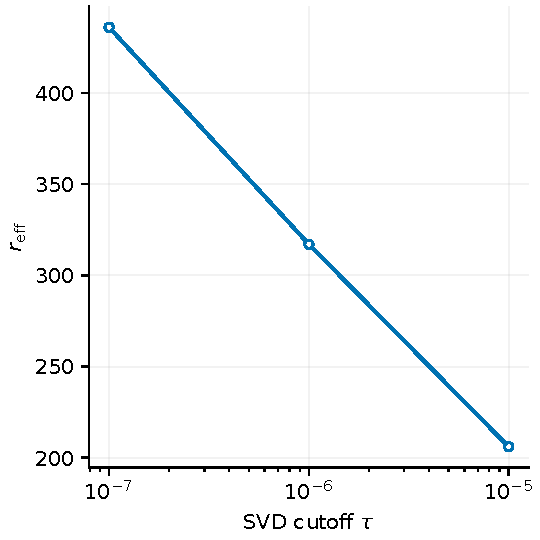
\includegraphics[width=\linewidth]
    {figures/fig10a.pdf}
\end{minipage}\hfill%
\begin{minipage}[t]{0.325\linewidth}
  \vspace{0pt}
  \centering
  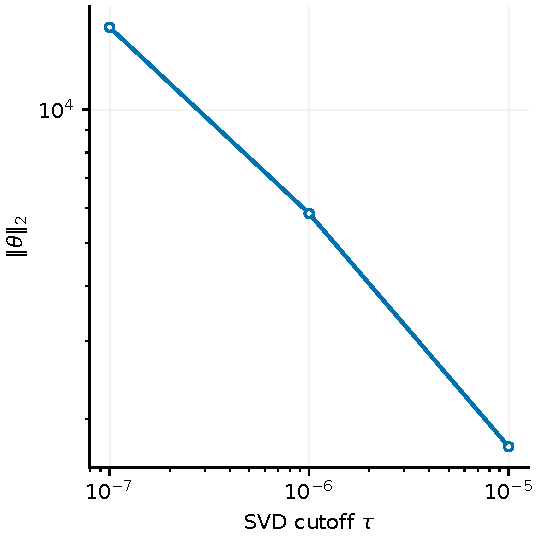
\includegraphics[width=\linewidth]
    {figures/fig10b.pdf}
\end{minipage}\hfill%
\begin{minipage}[t]{0.325\linewidth}
  \vspace{0pt}
  \centering
  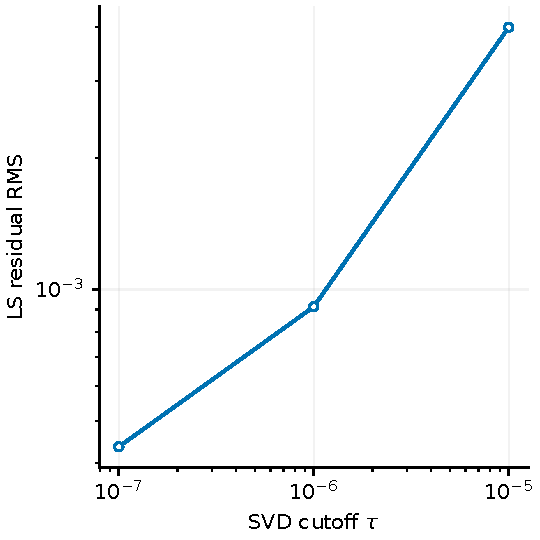
\includegraphics[width=\linewidth]
    {figures/fig10c.pdf}
\end{minipage}
\caption{Cutoff study: effective rank (left), original coefficient norm $\|\theta\|_2$ (center),
and RMS of the complete normalized least-squares residual (right). Here $z=D\theta$ is the column-equilibrated variable and the plotted norm is measured after recovery $\theta=D^{-1}z$. The cutoff is applied to the column-equilibrated system. These truncated-SVD solves are not directly covered by the exact least-squares quasi-optimality theorem on the original trial space.}
\label{fig:p5-cutoff-algebraic}
\end{figure}

\begin{figure}[!htbp]
\centering
\begin{minipage}{.45\linewidth}\centering
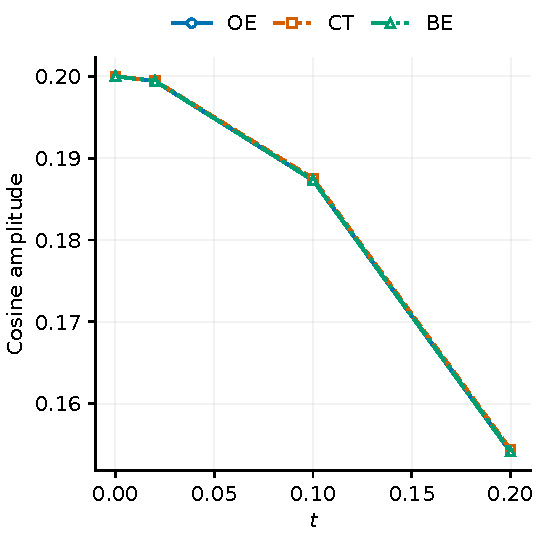
\includegraphics[width=0.90\linewidth]{figures/fig11a.pdf}
\end{minipage}\hfill
\begin{minipage}{.45\linewidth}\centering
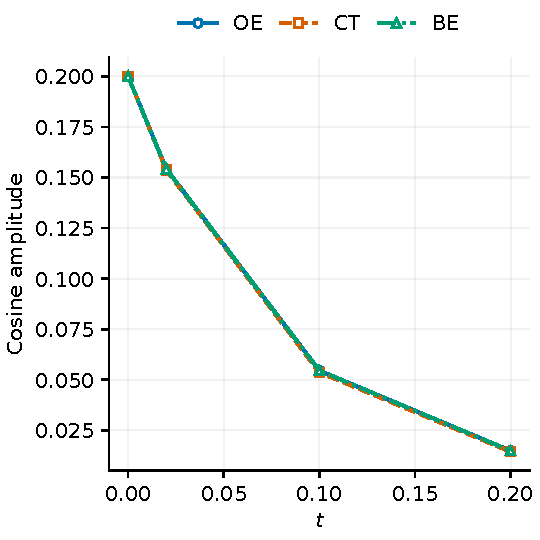
\includegraphics[width=0.90\linewidth]{figures/fig11b.pdf}
\end{minipage}
\caption{Cosine-mode amplitude for periodic transport with seed 11: $\varepsilon=1$ (left) and $10^{-3}$ (right). OE is compared with the continuous-time and same-step backward-Euler transport references at the saved output times.}
\label{fig:transient-amplitude}
\end{figure}

\begin{figure}[!htbp]
\centering
\begin{minipage}{.45\linewidth}\centering
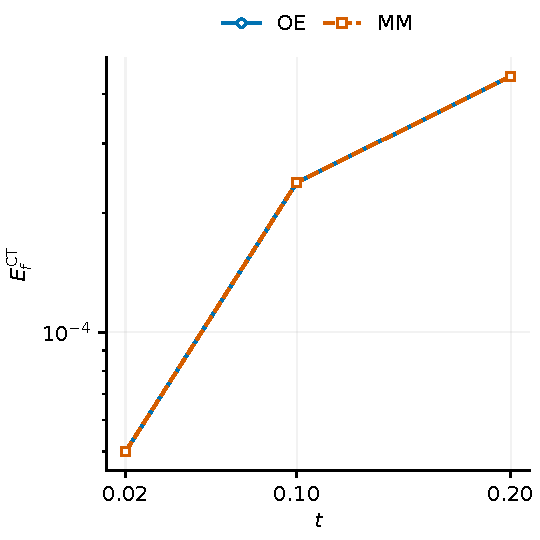
\includegraphics[width=0.90\linewidth]{figures/fig12a.pdf}
\end{minipage}\hfill
\begin{minipage}{.45\linewidth}\centering
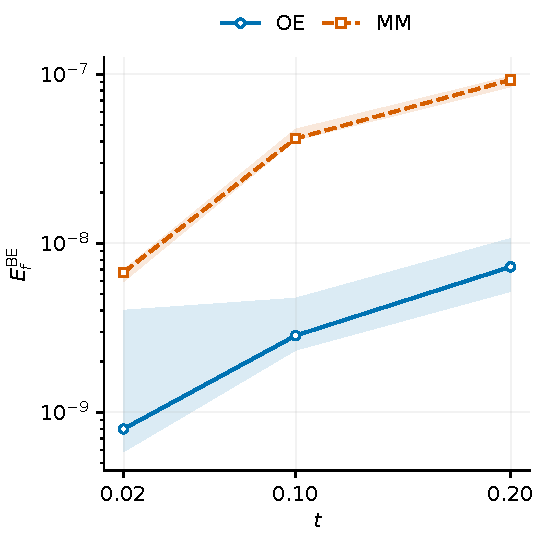
\includegraphics[width=0.90\linewidth]{figures/fig12b.pdf}
\end{minipage}
\par\smallskip
\begin{minipage}{.45\linewidth}\centering
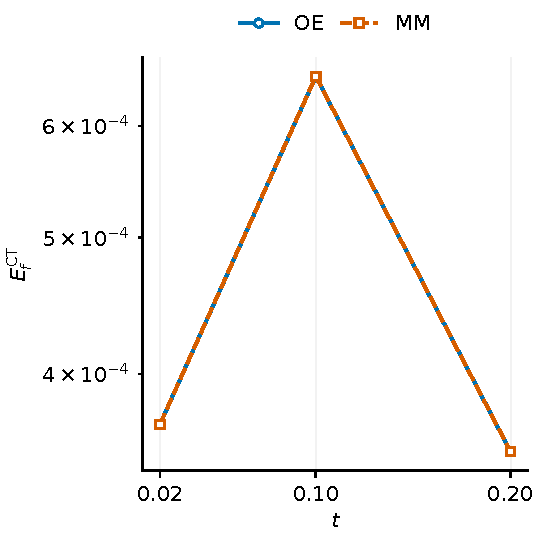
\includegraphics[width=0.90\linewidth]{figures/fig12c.pdf}
\end{minipage}\hfill
\begin{minipage}{.45\linewidth}\centering
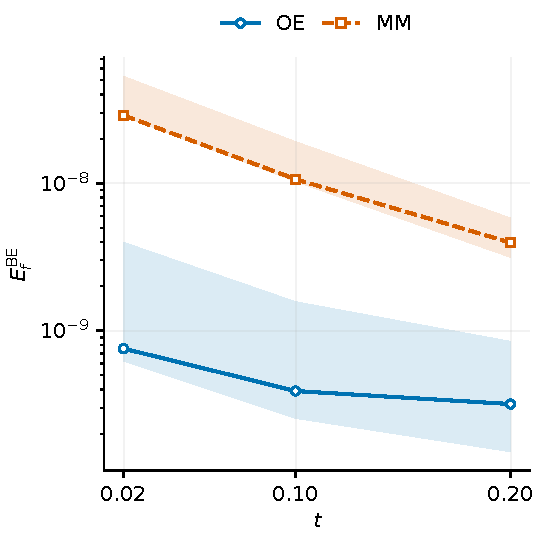
\includegraphics[width=0.90\linewidth]{figures/fig12d.pdf}
\end{minipage}
\caption{OE/MM kinetic errors for periodic transport at the three evaluated output times with $\Delta t=0.002$ and 256 coefficients per method. Rows correspond to $\varepsilon=1$ and $10^{-3}$; columns use the CT reference (left) and same-step BE reference (right). Curves show three-seed medians and bands show the minimum-maximum range.}
\label{fig:transient-error-evolution}
\end{figure}


\begin{figure}[!htbp]
\centering
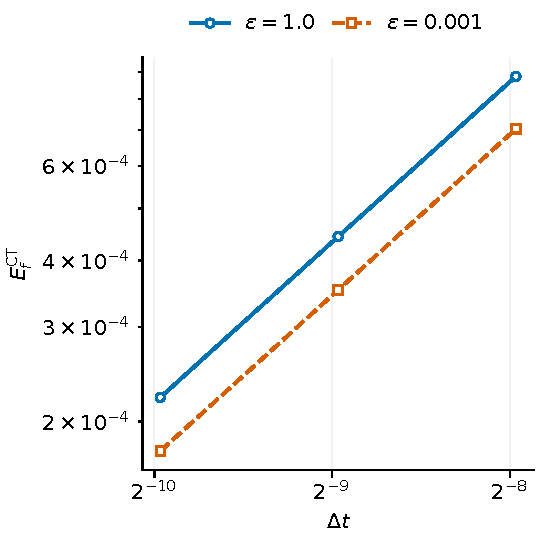
\includegraphics[width=0.75\linewidth]{figures/fig13.pdf}
\caption{Backward-Euler time refinement for periodic transport with seed 11 against the continuous-time transport reference at $T=0.2$. The steps $\Delta t=0.004,0.002,0.001$ correspond to 50, 100, and 200 time steps.}
\label{fig:time-refinement}
\end{figure}

\begin{figure}[!htbp]
\centering
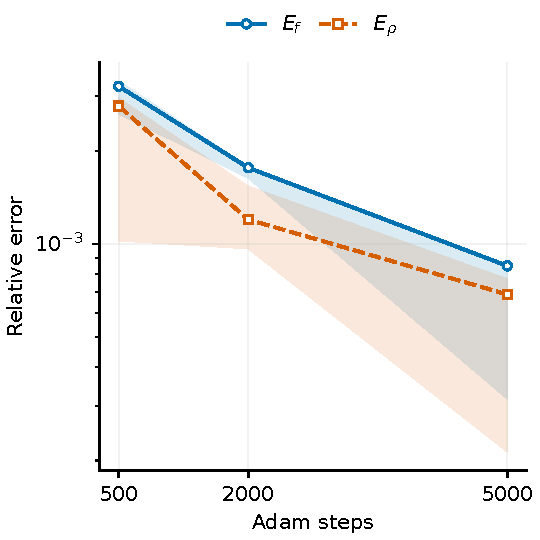
\includegraphics[width=0.8\linewidth]{figures/fig14.pdf}
\caption{Hard-parity OE-APNN P1 retraining at $\varepsilon=10^{-3}$ with 4096 interior and 1024 boundary phase samples. Medians and minimum--maximum bands use seeds 7, 11, 17. Only completed three-seed budgets are shown. Kinetic and density errors are plotted on a shared axis.}
\label{fig:apnn-hard-parity-p1}
\end{figure}

\begin{figure}[!htbp]
\centering
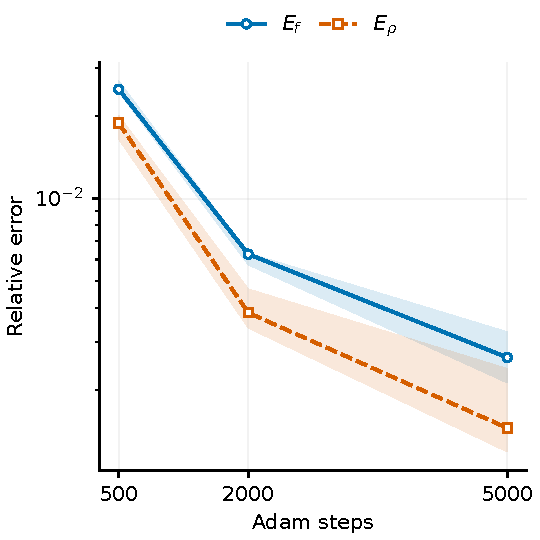
\includegraphics[width=0.8\linewidth]{figures/fig15.pdf}
\caption{Hard-parity OE-APNN P3 retraining at $\varepsilon=10^{-3}$ with 4096 interior and 1024 boundary phase samples. Medians and minimum--maximum bands use seeds 7, 11, 17. Only completed three-seed budgets are shown. Kinetic and density errors are plotted on a shared axis.}
\label{fig:apnn-hard-parity-p3}
\end{figure}
